%%%%%%%%%%%%%%%%%%%%
\subsection{2.3~~线性表的链式存储}
\begin{frame}\ft{\subsecname}
\begin{dingyi}[链式存储]
用一组任意的存储单元存储线性表中的数据元素。
用这种方法存储的线性表简称线性链表。
\end{dingyi}

\pause 
\begin{itemize}
\item[$\diamond$]
存储链表中结点的存储单元可以是连续的,也可以是不连续的,甚至是零散分布在内存中的任意位置上的。
\item[$\diamond$]
链表中的逻辑顺序和物理顺序不一定相同。
\end{itemize}•
\end{frame}


\begin{frame}\ft{\subsecname}
\begin{figure}
\centering
\begin{tikzpicture}
\foreach \i in {1,2}
\filldraw[very thick,fill=black!10] (\i-1,0)rectangle(\i,1);
\node [] at (0.5,0.5) {data};
\node [] at (1.5,0.5) {next};
\node [right] at (3.5,1) {data: 数据域,存放结点的值};
\node [right] at (3.5,0.2) {next: 指针域,存放结点的直接后继的地址};
\end{tikzpicture}
\end{figure}


\begin{itemize}
\item[$\diamond$]
链表是通过每个结点的指针域将线性表的$n$个结点按其逻辑次序链接在一起的。
\item[$\diamond$]
每一个结点只包含一个指针域的链表,称为单链表。
\item[$\diamond$]
为操作方便,总在链表的第一个结点之前附设一个头结点(头指针)head指向第一个结点。头结点的数据域可以不存储任何信息(或链表长度等信息)。
\item[$\diamond$]
单链表由表头唯一确定,因此单链表可用头指针的名字来命名。
\end{itemize}•
\end{frame}

\begin{frame}\ft{\subsecname}
 \begin{figure}
\centering
\begin{tikzpicture}
\node [right] at (0,6.5) {例1:线性表$L=(bat,cat,eat,fat,hat)$};

\pause 

\foreach \i in {1,4,7} {
\filldraw[thick,fill=red!20,rounded corners] (\i-1,2)rectangle(\i+1,3);
\draw[thick](\i-1+1.33,2)--(\i-1+1.33,3);
\filldraw[thick,fill=red!20,rounded corners] (\i-1,0.5)rectangle(\i+1,1.5);
\draw[thick](\i-1+1.33,.5)--(\i-1+1.33,1.5);
}
\foreach \i in {1,4} {
\draw[thick,->] (\i-1+1.67,2.5)--(\i+2,2.5);
\draw[thick,->] (\i-1+1.67,1)--(\i+2,1);
}

\draw[thick,->] (6+1.67,2.5)--(6+2.3,2.5)--(6+2.3,1.75)--(0.67,1.75)--(0.67,1.5);
\draw[thick,->] (6+1.67,1)--(6+2.5,1)--(6+2.5,0.5);
\draw[thick] (6+2.2,0.4)--(6+2.5,0.5)--(6+2.8,.6);
\draw[thick] (6+2.2,0.4)--(6+2.2,0.3);
\draw[thick] (6+2.5,0.5)--(6+2.5,0.3);
\draw[thick] (6+2.8,0.6)--(6+2.8,0.3);

\node [above] at (0.6,3) {head};
\node [] at (3+0.6,2.5) {bat};
\node [] at (6+0.6,2.5) {cat};
\node [] at (0.6,1) {eat};
\node [] at (3+0.6,1) {fat};
\node [] at (6+0.6,1) {hat};

\pause 

\foreach \i in {1,2,...,14} {
\filldraw[fill=blue!20] (10,\i*0.5-0.5)rectangle(11.5,\i*0.5);
}
\node [] at (10.75,6.75) {$\cd$};
\node [] at (10.75,6.25) {hat};         
\node [left] at (10,6.25) {$1100$};
\node [] at (10.75,5.75) {null};
\node [] at (10.75,5.25) {$\cd$};
\node [] at (10.75,4.75) {cat};        
\node [left] at (10,4.75) {$1300$};
\node [] at (10.75,4.25) {$1305$};
\node [] at (10.75,3.75) {eat};     \node [left] at (10,3.75) {1305};
\node [] at (10.75,3.25) {$3700$};
\node [] at (10.75,2.75) {$\cd$};
\node [] at (10.75,2.25) {bat};
\node [] at (10.75,1.75) {$1300$};
\node [] at (10.75,1.25) {fat};    
\node [left] at (10,1.25) {$3700$};
\node [] at (10.75,0.75) {$1100$};
\node [] at (10.75,0.25) {$\cd$};
\end{tikzpicture}
\end{figure}
\end{frame}


\begin{frame}[fragile]\ft{\subsecname}
\begin{block}{结点的描述与实现}
  \lstinputlisting[language=C,linerange={11-15}]
                  {Chapters/Ch02/Code/LinkList/LinkList.h}
\end{block}
\end{frame}

\begin{frame}[fragile]\ft{\subsecname}
\begin{block}{结点的实现}
结点是通过动态分配和释放来实现的,即需要时分配,不需要时释放。
\begin{lstlisting}[frame=no,backgroundcolor=\color{red!0!green!0!blue!0}]
malloc(), realloc(), sizeof(), free();
\end{lstlisting}
\pause 
\begin{itemize}
\item[$\diamond$]
动态分配
\begin{lstlisting}[frame=no,backgroundcolor=\color{red!0!green!0!blue!0}]
p=(LNode*)malloc(sizeof(LNode));
\end{lstlisting}
分配了一个类型为{\ttfamily LNode}的结点变量的空间,并将其首地址放入指针变量{\ttfamily p}中。\\[0.1in]
\item[$\diamond$]
动态释放
\begin{lstlisting}[frame=no,backgroundcolor=\color{red!0!green!0!blue!0}]
free(p);
\end{lstlisting}
系统回收由指针变量{\ttfamily p}指向的内存区。
\end{itemize}•
\end{block}
\end{frame}

%% \begin{frame}[fragile]\ft{常用操作}
%% \begin{itemize}
%% \item[(1)] 结点的赋值
%% \begin{figure}
\centering
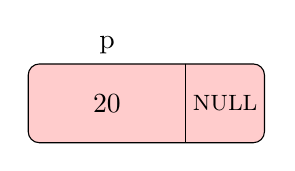
\begin{tikzpicture}
  \filldraw[fill=red!20,rounded corners](0,0)rectangle(3,1); 
  \node [] at (1,0.5) {20};
  \draw(2,0)rectangle(2,1); 
  \node [] at (2.5,0.5) {\footnotesize NULL};
  \node [above] at (1,1) {p};
\end{tikzpicture}
\end{figure}

%% \begin{figure}
\centering
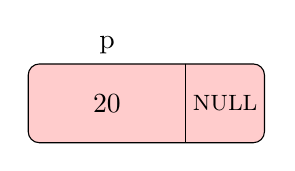
\begin{tikzpicture}
  \filldraw[fill=red!20,rounded corners](0,0)rectangle(3,1); 
  \node [] at (1,0.5) {20};
  \draw(2,0)rectangle(2,1); 
  \node [] at (2.5,0.5) {\footnotesize NULL};
  \node [above] at (1,1) {p};
\end{tikzpicture}
\end{figure}

%% \end{itemize}
 
%% \end{frame}


\begin{frame}[fragile]\ft{\subsecname}\fst{常用操作}
\begin{itemize}
\item[(2)] 常见的指针操作
\begin{figure}
\centering
\begin{tikzpicture}[scale=1.5]
\def \x{0.5}
\foreach \d in {0,4}{
\filldraw[fill=red!20,rounded corners](\d+0,0)rectangle(\d+2*\x,\x);  
\draw (\d+1.33*\x,0)rectangle(\d+1.33*\x,\x);  
\node [] at (\d+0.67*\x,0.5*\x) {a};
\node [above] at (\d+0.67*\x,2*\x) {p};
\draw[->,line width=1.5pt](\d+0.67*\x,2*\x)--(\d+0.67*\x,1.1*\x);
\draw[->,line width=1.5pt](\d-1*\x,0.5*\x)--(\d+0*\x,0.5*\x);
\draw[->,line width=1.5pt](\d+1.5*\x,0.5*\x)--(\d+2.5*\x,0.5*\x);
}

\def \d{4}
\node[below] at (\x,0) {操作前};
\node[below] at (\d+\x,0) {操作后};
\node [above] at (\d-\x,2*\x) {q};
\draw[->,line width=1.5pt] (\d-1*\x,2*\x)--(\d-1*\x,\x)--(\d+0*\x,\x);

\end{tikzpicture}
\caption{q=p}
\end{figure}
\pause 
\begin{figure}
\centering
\begin{tikzpicture}[scale=1.5]
\def \x{0.5}
\foreach \d in {0,4}{
\filldraw[fill=red!20,rounded corners](\d+0,0)rectangle(\d+2*\x,\x);  
\draw (\d+1.33*\x,0)--(\d+1.33*\x,\x); 
\filldraw[fill=red!20,rounded corners](\d+3*\x,0)rectangle(\d+5*\x,\x);  
\draw (\d+3*\x+1.67*\x,0)--(\d+3*\x+1.67*\x,\x); 

 
\node [] at (\d+0.67*\x,0.5*\x) {a};
\node [] at (\d+3.67*\x,0.5*\x) {b};
\node [above] at (\d+0.67*\x,2*\x) {p};
\draw[->,line width=1.5pt](\d+0.67*\x,2*\x)--(\d+0.67*\x,1.1*\x);
\draw[->,line width=1.5pt](\d-1*\x,0.5*\x)--(\d+0*\x,0.5*\x);
\draw[->,line width=1.5pt](\d+1.5*\x,0.5*\x)--(\d+3*\x,0.5*\x);
}

\def \d{4}
\node[below=4pt] (before) at (3*\x,0) {操作前};
\node[below=4pt] (after) at (\d+3*\x,0) {操作后};
\node [above] at (\d+3.67*\x,2*\x) {q};
\draw[->,line width=1.5pt] (\d+3.67*\x,2*\x)--(\d+3.67*\x,1.1*\x);
\end{tikzpicture}
\caption{q = p->next}
\end{figure}

\end{itemize}
 
\end{frame}

\begin{frame}[fragile]\ft{\subsecname}\fst{常用操作}
\begin{figure}
\centering
\begin{tikzpicture}
\def \x{0.5}
\foreach \d in {0,5}{
\filldraw[fill=red!20](\d+0,0)rectangle(\d+\x,\x);  
\filldraw[fill=red!20](\d+\x,0)rectangle(\d+2*\x,\x); 
\filldraw[fill=red!20](\d+3*\x,0)rectangle(\d+4*\x,\x);  
\filldraw[fill=red!20](\d+4*\x,0)rectangle(\d+5*\x,\x); 

\node [] at (\d+0.5*\x,0.5*\x) {a};
\node [] at (\d+3.5*\x,0.5*\x) {b};

\draw[->](\d-1*\x,0.5*\x)--(\d+0*\x,0.5*\x);
\draw[->](\d+1.5*\x,0.5*\x)--(\d+3*\x,0.5*\x);
}
\def\d{0}
\draw[->](\d+0.5*\x,2*\x)--(\d+0.5*\x,\x);
\node [above] at (\d+0.5*\x,2*\x) {p};


\def \d{5}
\node[below] at (3*\x,0) {操作前};
\node[below] at (\d+3*\x,0) {操作后};
\node [above] at (\d+3.5*\x,2*\x) {p};
\draw[->] (\d+3.5*\x,2*\x)--(\d+3.5*\x,\x);
\end{tikzpicture}
\caption{p=p-\textgreater next;}
\end{figure}
\pause 
\begin{figure}
\centering

\begin{tikzpicture}
\def \x{0.5}

\foreach \d in {0,5}{
\filldraw[fill=red!20](\d+0,0)rectangle(\d+\x,\x);  
\filldraw[fill=red!20](\d+\x,0)rectangle(\d+2*\x,\x); 
\filldraw[fill=red!20](\d+3*\x,0)rectangle(\d+4*\x,\x);  
\filldraw[fill=red!20](\d+4*\x,0)rectangle(\d+5*\x,\x); 
\filldraw[fill=red!20](\d+3*\x,-1.5*\x)rectangle(\d+4*\x,-0.5*\x);  
\filldraw[fill=red!20](\d+4*\x,-1.5*\x)rectangle(\d+5*\x,-0.5*\x); 

 
\node [] at (\d+0.5*\x,0.5*\x) {a};
\node [] at (\d+3.5*\x,0.5*\x) {b};
\node [] at (\d+3.5*\x,-1*\x) {c};
\node [left] at (\d+1.5*\x,-1*\x) {p};

\draw[->](\d-1*\x,0.5*\x)--(\d+0*\x,0.5*\x);
\draw[->](\d+1.5*\x,-1*\x)--(\d+3*\x,-1*\x);

\draw[->](\d+0.5*\x,2*\x)--(\d+0.5*\x,\x);
\node [above] at (\d+0.5*\x,2*\x) {q};
}

\def\d{0}
\draw[->](\d+1.5*\x,0.5*\x)--(\d+3*\x,0.5*\x);
 
\def\d{5}
\draw[->](\d+1.5*\x,0.5*\x)--(\d+2.5*\x,0.5*\x)--(\d+2.5*\x,-0.5*\x)--(\d+3*\x,-0.5*\x);

\def \d{5}
\node[below] at (3*\x,-1.5*\x) {操作前};
\node[below] at (\d+3*\x,-1.5*\x) {操作后};
%\node [above] at (\d+3.5*\x,2*\x) {q};
%\draw[->] (\d+3.5*\x,2*\x)--(\d+3.5*\x,\x);

\end{tikzpicture}
\caption{q-\textgreater next=p;}
\end{figure}

 
 
\end{frame}


\begin{frame}[fragile]\ft{\subsecname}\fst{常用操作}
 \begin{figure}
\centering

\begin{tikzpicture}
\def \x{0.5}

\foreach \c in {0,-2.5}{
\foreach \d in {0,5}{
\filldraw[fill=red!20](\d+0,\c+0)rectangle(\d+\x,\c+\x);  
\filldraw[fill=red!20](\d+\x,\c+0)rectangle(\d+2*\x,\c+\x); 
\filldraw[fill=red!20](\d+3*\x,\c+0)rectangle(\d+4*\x,\c+\x);  
\filldraw[fill=red!20](\d+4*\x,\c+0)rectangle(\d+5*\x,\c+\x); 

 
\draw[->](\d-1*\x,\c+0.5*\x)--(\d+0*\x,\c+0.5*\x);

\ifthenelse{  0 = \d \AND   -2 = \c}{
\draw[->](\d+1.5*\x,\c+0.5*\x)--(\d+1.5*\x,\c-0.5*\x)
--(5+0.5*\x,\c-0.5*\x)--(5+0.5*\x,\c);
}{
\draw[->](\d+1.5*\x,\c+0.5*\x)--(\d+3*\x,\c+0.5*\x);
}

\draw[->](\d+4.5*\x,\c+0.5*\x)--(\d+5.5*\x,\c+0.5*\x);
}
\node [] at (3.7,\c+0.5*\x) {$\cd\cd$};


\def\d{0}
\node [] at (\d+0.5*\x,\c+0.5*\x) {a};
\node [] at (\d+3.5*\x,\c+0.5*\x) {b};

\draw[->](\d+0.5*\x,\c+2*\x)--(\d+0.5*\x,\c+\x);
\node [above] at (\d+0.5*\x,\c+2*\x) {q};

\def\d{5}
\node [] at (\d+0.5*\x,\c+0.5*\x) {x};
\node [] at (\d+3.5*\x,\c+0.5*\x) {y};


\def \d{5}
\ifthenelse{  0 = \c}{
\node[below] at (7*\x,\c+0) {操作前};
}{
\node[below] at (7*\x,\c-1*\x) {操作后};
}

\node [above] at (\d+0.5*\x,\c+2*\x) {p};
\draw[->] (\d+0.5*\x,\c+2*\x)--(\d+0.5*\x,\c+\x);
}
\end{tikzpicture}
\caption{q-\textgreater next=p;}
\end{figure}
 
\end{frame}

\begin{frame}[fragile]\ft{\subsecname}\fst{常用操作}
\begin{figure}
\centering

\begin{tikzpicture}
\def \x{0.5}

\foreach \d in {0,5}{
\foreach \c in {0,-1}{
\filldraw[fill=red!20](\d+0,\c+0)rectangle(\d+\x,\c+\x);  
\filldraw[fill=red!20](\d+\x,\c+0)rectangle(\d+2*\x,\c+\x); 
\filldraw[fill=red!20](\d+3*\x,\c+0)rectangle(\d+4*\x,\c+\x);  
\filldraw[fill=red!20](\d+4*\x,\c+0)rectangle(\d+5*\x,\c+\x); 
 
\ifthenelse{0 = \c}{
\node [] at (\d+0.5*\x,\c+0.5*\x) {a};
\node [] at (\d+3.5*\x,\c+0.5*\x) {b};
}{
\node [] at (\d+0.5*\x,\c+0.5*\x) {x};
\node [] at (\d+3.5*\x,\c+0.5*\x) {y};
}

\draw[->](\d-1*\x,\c+0.5*\x)--(\d+0*\x,\c+0.5*\x);
\draw[->](\d+4.5*\x,\c+0.5*\x)--(\d+5.5*\x,\c+0.5*\x);

\ifthenelse{0 = \c \AND 5 = \d}{
\draw[->](\d+1.5*\x,\c+0.5*\x)--(\d+2.5*\x,\c+0.5*\x)
--(\d+2.5*\x,\c-\x)--(\d+3*\x,\c-\x);
}{
\draw[->](\d+1.5*\x,\c+0.5*\x)--(\d+3*\x,\c+0.5*\x);
}

\ifthenelse{0 = \c}{
\draw[->](\d+0.5*\x,\c+2*\x)--(\d+0.5*\x,\c+\x);
\node [above] at (\d+0.5*\x,\c+2*\x) {q};
}{}

\ifthenelse{-1 = \c}{
\node [left] at (\d-\x,\c+0.5*\x) {p};
}{}

}
\ifthenelse{0 = \d}{
\node [below] at (\d+2.5*\x,-2*\x) {操作前};
}{
\node [below] at (\d+2.5*\x,-2*\x) {操作后};
}

}
\end{tikzpicture}
\caption{q-\textgreater next=p-\textgreater next;}
\end{figure} 
\end{frame}


\begin{frame}[fragile]\ft{\subsecname}\fst{常用操作}
\begin{figure}
\centering

\begin{tikzpicture}
\def \x{0.5}

\foreach \c in {0,-2.5}{
\foreach \d in {0,5}{
\filldraw[fill=red!20](\d+0,\c+0)rectangle(\d+\x,\c+\x);  
\filldraw[fill=red!20](\d+\x,\c+0)rectangle(\d+2*\x,\c+\x); 
\filldraw[fill=red!20](\d+3*\x,\c+0)rectangle(\d+4*\x,\c+\x);  
\filldraw[fill=red!20](\d+4*\x,\c+0)rectangle(\d+5*\x,\c+\x); 

 
\draw[->](\d-1*\x,\c+0.5*\x)--(\d+0*\x,\c+0.5*\x);

\ifthenelse{  0 = \d \AND   -2 = \c}{
\draw[->](\d+1.5*\x,\c+0.5*\x)--(\d+1.5*\x,\c-0.5*\x)
--(5+3.5*\x,\c-0.5*\x)--(5+3.5*\x,\c);
}{
\draw[->](\d+1.5*\x,\c+0.5*\x)--(\d+3*\x,\c+0.5*\x);
}

\draw[->](\d+4.5*\x,\c+0.5*\x)--(\d+5.5*\x,\c+0.5*\x);
}
\node [] at (3.7,\c+0.5*\x) {$\cd\cd$};


\def\d{0}
\node [] at (\d+0.5*\x,\c+0.5*\x) {a};
\node [] at (\d+3.5*\x,\c+0.5*\x) {b};

\draw[->](\d+0.5*\x,\c+2*\x)--(\d+0.5*\x,\c+\x);
\node [above] at (\d+0.5*\x,\c+2*\x) {q};

\def\d{5}
\node [] at (\d+0.5*\x,\c+0.5*\x) {x};
\node [] at (\d+3.5*\x,\c+0.5*\x) {y};


\def \d{5}
\ifthenelse{  0 = \c}{
\node[below] at (7*\x,\c+0) {操作前};
}{
\node[below] at (7*\x,\c-1*\x) {操作后};
}

\node [above] at (\d+0.5*\x,\c+2*\x) {p};
\draw[->] (\d+0.5*\x,\c+2*\x)--(\d+0.5*\x,\c+\x);
}
\end{tikzpicture}
\caption{q-\textgreater next=p-\textgreater next;}
\end{figure}
  
\end{frame}

\begin{frame}\ft{\subsecname}\fst{单链表的整表创建}
  \begin{itemize}
  \item  顺序存储结构的创建,就是一个数组的初始化。而单链表则不同,它可以很散,是一个动态结构。
  \item 对每个链表而言,它所占用空间的大小和位置不需要预先分配,可根据系统的情况和实际需求即时生成。
  \end{itemize}
  
  所以创建单链表的过程就是一个动态生成链表的过程,即从空表的初始状态起,一次建立各元素结点,并逐个插入链表。
\end{frame}


\begin{frame}\ft{\subsecname}\fst{单链表的整表创建} 
动态地建立单链表的常用方法有两种:
\begin{itemize}
\item[$\diamond$]
头插入法
\item[$\diamond$]
尾插入法
\end{itemize}•
\end{frame}

\begin{frame}\ft{\subsecname}\fst{单链表的整表创建(头插入法)}
  \begin{itemize}
  \item 声明一结点{\ttfamily p}和计数器变量{\ttfamily i}
  \item 初始化一空链表{\ttfamily L}
  \item 让{\ttfamily L}的头结点的指针指向{\ttfamily NULL},即建立一个带头结点的单链表
  \item 循环
    \begin{itemize}
    \item 生成一个新结点赋值给{\ttfamily p}\\[0.1in]
    \item 随机生成一个数赋给{\ttfamily p}的数据域{\ttfamily p->data}\\[0.1in]
    \item 将{\ttfamily p}插入到头结点与前一新结点之间
    \end{itemize}
  \end{itemize}
\end{frame}

\begin{frame}[fragile]\ft{\subsecname}\fst{单链表的整表创建(头插入法)}

  %% \begin{lstlisting}[language=C,frame=tb,backgroundcolor=\color{red!10}]
//`随机生成n个元素,建立带表头结点的单链表L`
void CreateLinkListHead(LinkList *L, int n){
  LinkList p;
  int i;
  srand(time(0));
  *L=(LinkList) malloc(sizeof(LNode));
  (*L)->next=NULL;
  LNode *head, *p;
  for(i=0;i<n;i++)
    p=(LinkList)malloc(sizeof(LNode));
    p->data=rand()%100+1;
    p->next=(*L)->next;
    (*L)->next=p;
}
\end{lstlisting}

  \lstinputlisting[
    language=C,
    linerange={3-5,7-14},
    frame=tb,
  ]{Chapters/Ch02/Code/LinkList/CreateLinkListHead.c}
\end{frame}

\begin{frame}\ft{\subsecname}\fst{单链表的整表创建(尾插入法)}
 头插入法建立链表虽然算法简单,但生成的链表中结点的次序和输入的顺序相反。若希望二者次序一致,可采用尾插法建表。该方法是将新结点插入到当前链表的表尾,使其成为当前链表的尾结点。
\end{frame}

\begin{frame}[fragile]\ft{\subsecname}\fst{单链表的整表创建(尾插入法)}
  
  %% \begin{lstlisting}[language=C,frame=tb,backgroundcolor=\color{red!10}]
void CreateLinkListTail(LinkList *L,int n){
  LinkList p,r;
  srand(time(0));
  *L=(LinkList)malloc(sizeof(LNode));
  r=*L;
  for(i=0;i<n;i++){
    p=(Lnode *)malloc(sizeof(LNode));
    p->data=rand()%100+1;
    r->next=p;
    r=p;
  }
  r->next=NULL;
}
\end{lstlisting}


  \lstinputlisting[
    language=C,
    linerange={3-5,7-15},
    frame=tb,
  ]{Chapters/Ch02/Code/LinkList/CreateLinkListTail.c}
\end{frame}

\begin{frame}\ft{\subsecname}\fst{单链表的查找}
\begin{enumerate}
\item 按序号查找
\item 按值查找
\end{enumerate}•
\end{frame}

\begin{frame}\ft{\subsecname}\fst{单链表的查找(按序号)}
 

对于单链表,不能像顺序表中那样直接按序号$i$访问结点,而只能从链表的头结点出发,沿指针域next逐个结点往下搜索,知道搜到第$i$个结点为止。因此,链表不是随机存储结构。

\vspace{0.2in}

设单链表长度为$n$,要查找第$i$个结点,仅当$1\le i \le n$时,$i$的值是合法的。
 
\end{frame}

\begin{frame}[fragile]\ft{\subsecname}\fst{单链表的查找(按序号)}
%% \begin{lstlisting}[language=C,frame=tb,backgroundcolor=\color{red!10}]
Status Get_Elem(LinkList L,int i,ElemType *e) {
  int j; LinkList p;
  p=L->next; j=1;
  while (p!=NULL&&j<i){
    p=p->next; j++;
  }
  if (!p || j>i) 
    return error; //`第i个元素不存在`
  *e=p->data;     //`取第i个元素的数据`
  return OK;
}
\end{lstlisting}
 

\lstinputlisting[
  language=C,
  linerange={3-15},
  frame=tb,
]{Chapters/Ch02/Code/LinkList/GetElem.c}

\end{frame}

\begin{frame}[fragile]\ft{\subsecname}\fst{单链表的查找(按序号)}
\begin{block}{移动指针{\tt p}的频度}
\[\left\{
\begin{array}{rl}
0\mbox{次},& i<1;\\[0.1in]
i-1\mbox{次}, & i  \in [1,n];\\[0.1in]
n\mbox{次}, & i>n.
\end{array}
\right.
~~\Rightarrow~~\mbox{时间复杂度为}O(n).
\] 
\end{block}

\end{frame}


\begin{frame}\ft{\subsecname}\fst{单链表的查找(按值)}
 
按值查找是在链表中,查找是否有结点值等于给定值key的结点?
\begin{itemize}
\item
若有,则返回首次找到的值为{\tt key}的结点的存储位置;
\item
否则返回{\tt NULL}。
\end{itemize}
查找时从开始结点出发,沿链表逐个将结点的值和给定值{\tt key}作比较。

\end{frame}

\begin{frame}[fragile]\ft{\subsecname}\fst{单链表的查找(按值)}
%% \begin{lstlisting}[language=C]
LinkList Locate_Node_Key(LinkList L,int key) {
  LinkList p=L->next;  
  while (p!=NULL&&p->data!=key)  p=p->next;  
  if (p->data==key) return p;
  else {
    printf("要查找的结点不存在!\n");
    return (NULL);
  }
}
\end{lstlisting}
 
\lstinputlisting[
  language=C,
  linerange={3-12},
  frame=tb,
]{Chapters/Ch02/Code/LinkList/LocateNodeKey.c}

\end{frame}

\begin{frame}[fragile]\ft{\subsecname}\fst{单链表的查找(按值)}

\begin{block}{平均时间复杂度}
算法的执行与形参{\tt key}有关,平均时间复杂度为$O(n)$。
\end{block}

\end{frame}


\begin{frame}\ft{\subsecname}\fst{插入结点}
 
插入运算是指将值为$e$的新结点插入到表的第$i$个结点的位置上,即插入到$a_{i-1}$与$a_i$之间。因此,必须首先找到$a_{i-1}$所在的结点$p$,然后生成一个数据域为$e$的新结点$q$,$q$作为$p$的直接后继。
\end{frame}

\begin{frame}[fragile]\ft{\subsecname}\fst{插入结点}
  \lstinputlisting[
    language=C,
    linerange={3-15},
    frame=tb,
  ]{Chapters/Ch02/Code/LinkList/InsertLNode.c}
%% \begin{lstlisting}[language=C]
void Insert_LNode(LinkList L, int i, ElemType e) {
  int j=0; LinkList p,q;  
  p=L->next;
  while (p!=NULL&&j<i-1){
    p=p->next;  j++;
  }
  if (j!=i-1) printf("i`太大或`i`为`0!\n");
  else {
    q=(LNode *)malloc(sizeof(LNode));
    q->data=e; q->next=p->next;
    p->next=q;;
  }
}
\end{lstlisting}
 
\end{frame}


\begin{frame}\ft{\subsecname}\fst{插入结点}

\begin{block}{平均时间复杂度}
设链表长度为$n$,合法的插入位置是$1\le i \le n$。
算法的时间主要耗费在移动指针$p$上,平均时间复杂度为$O(n)$。
\end{block}

\end{frame}


\begin{frame}\ft{\subsecname}\fst{删除结点}
\begin{itemize}
\item[$\diamond$]
按序号删除:删除单链表中的第$i$个结点。\\[0.2in]
\item[$\diamond$]
按值删除:删除单链表中值为key的第一个结点。
\end{itemize}
\end{frame}


\begin{frame}\ft{\subsecname}\fst{删除结点(按序号)}
 \begin{itemize}
\item 为了删除第$i$个结点$a_i$,必须找到结点的存储地址。
\item 该存储地址在其直接前驱结点$a_{i-1}$的next域中,因此必须首先找到$a_{i-1}$的存储位置$p$,
然后令{\ttfamily p->next}指向$a_i$的直接后继结点,即把$a_i$从链上摘下来。
\item
最后释放结点$a_i$的空间,将其归还给“存储池”。
\end{itemize}•
 
 
 设单链表长度为$n$,则删去第$i$个结点仅当$1\le i \le n$时是合法的。当$i=n+1$时,虽然被删结点不存在,但其前驱结点却存在,是终端结点。故判断条件之一是{\ttfamily p->next!=NULL}。
 
\end{frame}

\begin{frame}[fragile]\ft{\subsecname}\fst{删除结点(按序号)}
  \lstinputlisting[
    language=C,
    linerange={3-14},
    frame=tb,
  ]{Chapters/Ch02/Code/LinkList/DeleteLNodeIndex.c}
  %% \begin{lstlisting}[language=C]
void Delete_LinkList_Index(LinkList L, int i) {
  int j=1; LNode *p, *q;  
  p=L; q=L->next;
  while (p->next!=NULL&&j<i){
    p=q; q=q->next;  j++;
  }
  if (j!=i) printf("i`太大或`i`为`0!\n");
  else {
     p->next=q->next; free(q);
  }
}
\end{lstlisting}

\end{frame}

\begin{frame}[fragile]\ft{\subsecname}\fst{删除结点(按序号)}
\begin{block}{时间复杂度}
时间复杂度为$O(n)$。
\end{block}

\end{frame}


\begin{frame}\ft{\subsecname}\fst{删除结点(按值)}

 
与按值查找相类似,首先要查找值为{\ttfamily key}的结点是否存在?
\begin{itemize}
\item 若存在,则删除;
\item 否则返回{\ttfamily NULL}。
\end{itemize}

\end{frame}

\begin{frame}[fragile]\ft{\subsecname}\fst{删除结点(按值)}
  \lstinputlisting[
    language=C,
    linerange={3-18},
    frame=tb,
  ]{Chapters/Ch02/Code/LinkList/DeleteLNodeKey.c}
  %% \begin{lstlisting}[language=C]
void Delete_LinkList_Key(LinkList L, int key) {
  LinkList p=L, q=L->next;  
  while (q!=NULL&&q->data!=key){
    p=q; q=q->next;   
  }
  if (q->data==key) {
    p->next=q->next; free(q);
  }
  else {
        printf("`要删除的结点不存在`!\n");
  }
}
\end{lstlisting}
 
\end{frame}

\begin{frame}[fragile]\ft{删除结点}\fst{按值删除}

  \begin{block}{时间复杂度}
    时间复杂度为$O(n)$。
  \end{block}
\end{frame}

\begin{frame}[fragile]\ft{\subsecname}\fst{删除结点}
链表实现插入和删除运算,无需移动结点,仅需修改指针,解决了顺序表的插入或删除操作需要移动大量元素的问题。
\end{frame}

\begin{frame}[fragile]\ft{\subsecname}\fst{删除多个结点(按值)}
\begin{block}{变形之一}
删除单链表中值为key的所有结点。
\end{block}
\pause 
\begin{block}{基本思想}
\begin{itemize}
\item
从单链表的第一个结点开始,对每个结点进行检查,若结点的值为{\ttfamily key},则删除之,
\item
然后检查下一个结点,直到所有的结点都检查。
\end{itemize}
\end{block}


\end{frame}


\begin{frame}[fragile]\ft{\subsecname}\fst{删除多个结点(按值)}
\begin{lstlisting}[language=C]
void Delete_LinkList_Node(LinkList L, int key) {
  LinkList p=L, q=L->next;  
  while (q!=NULL){
    if (q->data!=key){
      p->next=q->next; free(q); q=p->next;
    } else {
      p=q; q=q->next;
    }
  }
}
 

\end{lstlisting}

 
\end{frame}

\begin{frame}[fragile]\ft{\subsecname}\fst{删除重复结点}
\begin{block}{变形之二}
删除单链表中所有值重复的结点,使得所有结点的值都不相同。
\end{block}
\pause 
\begin{block}{基本思想}
从单链表的第一个结点开始,对每个结点进行检查:
\begin{itemize}
\item
检查链表中该结点的所有后继结点,只要有值和该结点的值相同,则删除之;
\item
然后检查下一个结点,直到所有的结点都检查。
\end{itemize}
\end{block}


\end{frame}


\begin{frame}[fragile]\ft{\subsecname}\fst{删除重复结点}


\begin{lstlisting}[language=C]
void Delete_LinkList_Value(LNode *L) {
  LinkList p=L->next, q, ptr;  
  while (p!=NULL){
    *q=p; *ptr=p->next;
    while(ptr!=NULL){
      if (ptr->data==p->data){
        q->next=ptr->next; free(ptr); ptr=q->next;
      } else {
        q=ptr; ptr=ptr->next;
      }
    }
    p=p->next;
  }
}
\end{lstlisting}
 
 
\end{frame}


\begin{frame}\ft{单链表的合并}
设有两个有序的单链表,它们的头指针分别为$La$、$Lb$,
将它们合并为以$Lc$为头指针的有序链表。 
\begin{figure}
\centering
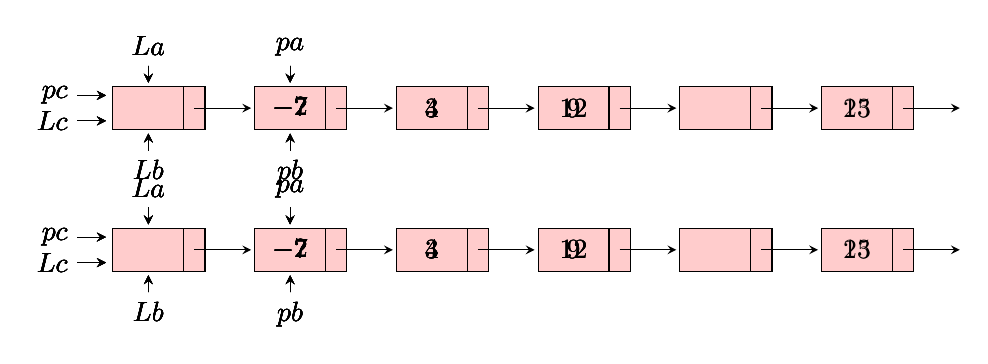
\begin{tikzpicture}[scale=0.9]
\def \x{1}
\def \y{0.6}

\foreach \c in {0,-2}{
\foreach \d in {0,2,4,6,8,10}{
\ifthenelse{  8 = \d }{
\node[left] at (\d+\x,\c+0.5*\y) {$\cd$};
}{
\filldraw[fill=red!20](\d+0,\c+0)rectangle(\d+\x,\c+\y);  
\filldraw[fill=red!20](\d+\x,\c+0)rectangle(\d+1.3*\x,\c+\y); 
}
\ifthenelse{  10 = \d}{

}{\draw[->,>=stealth] (\d+1.15*\x,\c+0.5*\y)--(\d+1.95*\x,\c+0.5*\y);}

\ifthenelse{ 0 = \c }{
\node[]at( 2.5,\c+0.5*\y){$-7$};
\node[]at( 4.5,\c+0.5*\y){$3$}; 
\node[]at( 6.5,\c+0.5*\y){$12$};
\node[]at(10.5,\c+0.5*\y){$23$};
\draw[->,>=stealth] (-.5*\x,\c+0.2*\y) node [left] {$Lc$}--(-0.1*\x,\c+0.2*\y);
\draw[->,>=stealth] (-.5,\c+0.8*\y) node[left] {$pc$}--(-.1*\x,\c+0.8*\y);
\draw[->,>=stealth] (2.5,\c+1.5*\y) node[above] {$pa$}--(2.5,\c+1.1*\y);
\draw[->,>=stealth] (0.5,\c+1.5*\y)node[above] {$La$} --(0.5,\c+1.1*\y);
}{
\node[]at( 2.5,\c+0.5*\y){$-2$};
\node[]at( 4.5,\c+0.5*\y){$4$}; 
\node[]at( 6.5,\c+0.5*\y){$9$};
\node[]at(10.5,\c+0.5*\y){$15$};
\draw[->,>=stealth] (2.5,\c-0.5*\y) node[below] {$pb$}--(2.5,\c-0.1*\y);
\draw[->,>=stealth] (0.5,\c-0.5*\y) node[below] {$Lb$}--(0.5,\c-0.1*\y);
}
}
}
\end{tikzpicture}
\caption{合并前的示意图}
\end{figure} 
\end{frame}


\begin{frame}\ft{\subsecname}\fst{单链表的合并}

  
\begin{figure}
\centering
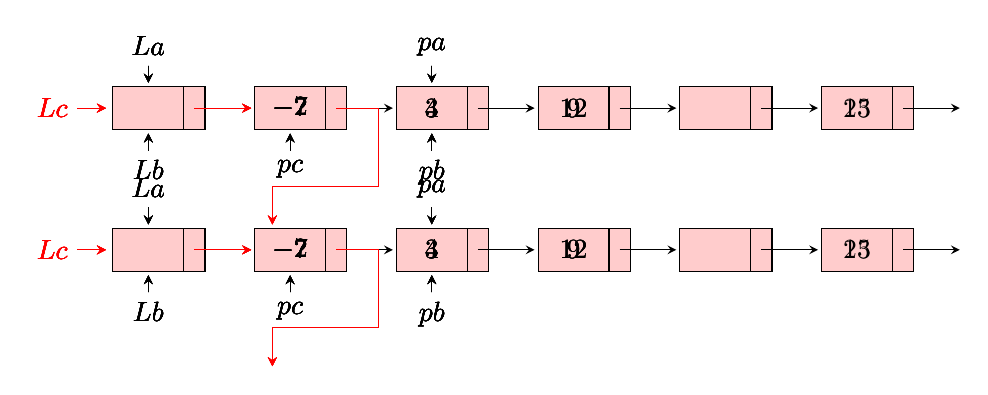
\begin{tikzpicture}[scale=0.9]
\def \x{1}
\def \y{0.6}

\foreach \c in {0,-2}{
\foreach \d in {0,2,4,6,8,10}{
\ifthenelse{  8 = \d }{
\node[left] at (\d+\x,\c+0.5*\y) {$\cd$};
}{
\filldraw[fill=red!20](\d+0,\c+0)rectangle(\d+\x,\c+\y);  
\filldraw[fill=red!20](\d+\x,\c+0)rectangle(\d+1.3*\x,\c+\y); 
}
\ifthenelse{   2 = \d \AND   0 = \c \OR  0 = \d \AND   0 = \c \OR 10 = \d}{

}{\draw[->,>=stealth] (\d+1.15*\x,\c+0.5*\y)--(\d+1.95*\x,\c+0.5*\y);}

\ifthenelse{ 0 = \c }{
\node[]at( 2.5,\c+0.5*\y){$-7$};
\node[]at( 4.5,\c+0.5*\y){$3$}; 
\node[]at( 6.5,\c+0.5*\y){$12$};
\node[]at(10.5,\c+0.5*\y){$23$};
\draw[->,>=stealth] (4.5,\c+1.5*\y) node[above] {$pa$}--(4.5,\c+1.1*\y);
\draw[->,>=stealth] (0.5,\c+1.5*\y)node[above] {$La$} --(0.5,\c+1.1*\y);
}{
\node[]at( 2.5,\c+0.5*\y){$-2$};
\node[]at( 4.5,\c+0.5*\y){$4$}; 
\node[]at( 6.5,\c+0.5*\y){$9$};
\node[]at(10.5,\c+0.5*\y){$15$};
\draw[->,>=stealth] (4.5,\c-0.5*\y) node[below] {$pb$}--(4.5,\c-0.1*\y);
\draw[->,>=stealth] (2.5,\c-0.5*\y) node[below] {$pc$}--(2.5,\c-0.1*\y);
\draw[->,>=stealth] (0.5,\c-0.5*\y) node[below] {$Lb$}--(0.5,\c-0.1*\y);
}

\ifthenelse{ 0 = \c }{
\draw[->,>=stealth,red] (-.5*\x,\c+0.5*\y) node [left] {$Lc$}--(-0.1,\c+0.5*\y);
\draw[->,>=stealth,red] (0+1.15*\x,\c+0.5*\y) --(0+1.95*\x,\c+0.5*\y);
\draw[->,>=stealth,red] (2+1.15*\x,\c+0.5*\y) --(2+1.75*\x,\c+0.5*\y)
--(2+1.75*\x,\c-2+2*\y)--(2+0.25*\x,\c-2+2*\y)--(2+0.25*\x,\c-2+1.1*\y);
}{}
}
}

\end{tikzpicture}
\caption{合并了值为$-7,-2$的结点后的示意图}
\end{figure} 

\pause 
\begin{itemize}
\item $pa,pb$分别是待考察的两个链表的当前结点;
\item $pc$是合并过程中合并的链表的最后一个结点。
\end{itemize}•
\end{frame}


\begin{frame}[fragile]\ft{\subsecname}\fst{单链表的合并}
\begin{lstlisting}[language=C]
LinkList Merge_Linklist(LinkList La, LinkList Lb){
  LinkList Lc,pa,pb,pc,ptr; 
  Lc=La; pc=La; pa=La->next; pb=Lb->next;
  while(pa!=NULL && pb!=NULL){
    if (pa->data<pb->data){
      pc->next=pa; pc=pa; pa=pa->next; }
    if (pa->data<pb->data){
      pc->next=pb; pc=pb; pb=pb->next; }
    if (pa->data==pb->data){
      pc->next=pa; pc=pa; pa=pa->next;
      ptr=pb; pb=pb->next; free(ptr); }
  }
  if(pa!=NULL) pc->next=pa;
  else pc->next=pb;
  free(Lb);
  return(Lc);
}
\end{lstlisting}
\end{frame}


\begin{frame}[fragile]\ft{\subsecname}\fst{单链表的合并}
\begin{block}{时间复杂度}
若$La,Lb$两个链表的长度分别为$m,n$,则链表合并的时间复杂度为$O(m+n)$。
\end{block}
\end{frame}
